%%%%%%%%%%%%%%%%%%%%%%%%%%%%%%%%%%%%%%%%%
% Jacobs Landscape Poster
% LaTeX Template
% Version 1.0 (29/03/13)
%
% Created by:
% Computational Physics and Biophysics Group, Jacobs University
% https://teamwork.jacobs-university.de:8443/confluence/display/CoPandBiG/LaTeX+Poster
% 
% Further modified by:
% Nathaniel Johnston (nathaniel@njohnston.ca)
%
% This template has been downloaded from:
% http://www.LaTeXTemplates.com
%
% 
% Masaryk University presentation themes were downloaded from:
% https://www.overleaf.com/gallery/tagged/muni
%
% and ported into Jacobs Landscape Poster by:
% Jumaidil Awal (ideal1st.here@googlemail.com)
% 
% Jacobs Landscape Poster License:
% CC BY-NC-SA 3.0 (http://creativecommons.org/licenses/by-nc-sa/3.0/)
%
% Masaryk University's fibeamer theme license:
% Copyright 2015  Vít Novotný <witiko@mail.muni.cz>
% Faculty of Informatics, Masaryk University (Brno, Czech Republic)
% under Latex Project Public License
%
%%%%%%%%%%%%%%%%%%%%%%%%%%%%%%%%%%%%%%%%%

%----------------------------------------------------------------------------------------
%	PACKAGES AND OTHER DOCUMENT CONFIGURATIONS
%----------------------------------------------------------------------------------------

\documentclass[final]{beamer}

\usepackage[scale=1.24]{beamerposter} % Use the beamerposter package for laying out the poster

%\usetheme{confposter} % Use the confposter theme supplied with this template
\usetheme[faculty=chemo]{fibeamer} % Uncomment to use Masaryk University's fibeamer theme instead.

%\setbeamercolor{block title}{fg=ngreen,bg=white} % Colors of the block titles
%\setbeamercolor{block body}{fg=black,bg=white} % Colors of the body of blocks
%\setbeamercolor{block alerted title}{fg=white,bg=dblue!70} % Colors of the highlighted block titles
%\setbeamercolor{block alerted body}{fg=black,bg=dblue!10} % Colors of the body of highlighted blocks
% Many more colors are available for use in beamerthemeconfposter.sty

%-----------------------------------------------------------
% Define the column widths and overall poster size
% To set effective sepwid, onecolwid and twocolwid values, first choose how many columns you want and how much separation you want between columns
% In this template, the separation width chosen is 0.024 of the paper width and a 4-column layout
% onecolwid should therefore be (1-(# of columns+1)*sepwid)/# of columns e.g. (1-(4+1)*0.024)/4 = 0.22
% Set twocolwid to be (2*onecolwid)+sepwid = 0.464
% Set threecolwid to be (3*onecolwid)+2*sepwid = 0.708

\newlength{\sepwid}
\newlength{\onecolwid}
\newlength{\twocolwid}
\newlength{\threecolwid}
\setlength{\paperwidth}{46.8in} % A0 width: 46.8in
\setlength{\paperheight}{33.1in} % A0 height: 33.1in
\setlength{\sepwid}{0.024\paperwidth} % Separation width (white space) between columns
\setlength{\onecolwid}{0.21\paperwidth} % Width of one column
\setlength{\twocolwid}{0.451\paperwidth} % Width of two columns
\setlength{\threecolwid}{0.678\paperwidth} % Width of three columns
%\setlength{\topmargin}{-0.5in} % Reduce the top margin size
%-----------------------------------------------------------

\usepackage{graphicx}  % Required for including images

\usepackage{booktabs} % Top and bottom rules for tables

\usepackage[absolute,overlay]{textpos}
  \setlength{\TPHorizModule}{1mm}
  \setlength{\TPVertModule}{1mm}

%----------------------------------------------------------------------------------------
%	TITLE SECTION 
%----------------------------------------------------------------------------------------

\title{What Makes Songs Popular?} % Poster title

\author{Cheng-Chun Lee, I Made Sanadhi Sutandi and Skander Hajri} % Author(s)

\institute{School of Computer and Communication Sciences, EPFL} % Institution(s)

%----------------------------------------------------------------------------------------

\begin{document}

\begin{textblock}{30}(925,30)
	
\includegraphics[width=6.3\linewidth]{img/epfl-logo.jpg}
\end{textblock}

\addtobeamertemplate{block end}{}{\vspace*{2ex}} % White space under blocks
\addtobeamertemplate{block example end}{}{\vspace*{2ex}} % White space under example blocks
\addtobeamertemplate{block alerted end}{}{\vspace*{2ex}} % White space under highlighted (alert) blocks

\setlength{\belowcaptionskip}{2ex} % White space under figures
\setlength\belowdisplayshortskip{2ex} % White space under equations
%\begin{darkframes} % Uncomment for dark theme, don't forget to \end{darkframes}
\begin{frame} % The whole poster is enclosed in one beamer frame

%==========================Begin Head===============================
  \begin{columns}
   \begin{column}{\linewidth}
    \vskip1cm
    \centering
    \usebeamercolor{title in headline}{\color{fg}\Huge{\textbf{\inserttitle}}\\[0.5ex]}
    \usebeamercolor{author in headline}{\color{fg}\Large{\insertauthor}\\[1ex]}
    \usebeamercolor{institute in headline}{\color{fg}\large{\insertinstitute}\\[1ex]}
    \vskip1cm
   \end{column}
   \vspace{1cm}
  \end{columns}
 \vspace{1cm}

%==========================End Head===============================

\begin{columns}[t] % The whole poster consists of three major columns, the second of which is split into two columns twice - the [t] option aligns each column's content to the top

\begin{column}{\sepwid}\end{column} % Empty spacer column

\begin{column}{\onecolwid} % The first column

%----------------------------------------------------------------------------------------
%	OBJECTIVES
%----------------------------------------------------------------------------------------

\begin{exampleblock}{Objective}
\begin{itemize}
\item Utilize \textbf{million songs dataset} to \textit{discover} \underline{interesting facts} prior to songs' popularity.
\end{itemize}

\end{exampleblock}

%----------------------------------------------------------------------------------------
%	INTRODUCTION
%----------------------------------------------------------------------------------------

\begin{exampleblock}{Introduction}

Song is one of the greatest creations of human kind in the course of history. Music has transformed itself into an area of industry and constantly changes over the time. Through this project, it is exciting for us to elaborate what factors influence songs' popularity at most.
\end{exampleblock}

\begin{exampleblock}{Million Songs Dataset}
We mainly use \textbf{Million Song Dataset} that has collection of audio features and metadata of popular and unpopular songs. In addition we also make use two additional datasets:
\begin{itemize}
\item The \textbf{musiXmatch} Dataset: Containing \textit{lyrics}.
\item The \textbf{Echo Nest Taste Profile} Subset: Containing \textit{users' profiles} with their play count.
\end{itemize}

Important fields of Million Song Dataset:
\begin{itemize}
\item \textit{track\_id}
The primary key identifier.
\item \textit{song\_hotttnesss} the popularity of a song measured between 0 - 1.
\end{itemize}
\end{exampleblock}

\begin{exampleblock}{Data Preprocessing}

\begin{itemize}
\item \textbf{Preprocessing} the big raw datasets using \textit{cluster operations} (Spark, Hadoop).
\item \textbf{Removing} \textit{unused attributes} based on analysis of features correlation; 52 $\rightarrow$ 28 features.
\item \textbf{Filtering} songs with \textit{missing songs hotness} entries; 1 million $\rightarrow$ 581,965 datapoints.
\item \textbf{Grouping} songs to \textit{popular} songs (popularity $\geq$ 0.8) and \textit{unpopular} songs (popularity $\leq$ 0.40)
\end{itemize}

\end{exampleblock}

%------------------------------------------------

% \begin{figure}
% \includegraphics[width=0.8\linewidth]{img/placeholder.jpg}
% \caption{Figure caption}
% \end{figure}

%----------------------------------------------------------------------------------------

\end{column} % End of the first column

\begin{column}{\sepwid}\end{column} % Empty spacer column

\begin{column}{\twocolwid} % Begin a column which is two columns wide (column 2)

\begin{columns}[t,totalwidth=\twocolwid] % Split up the two columns wide column

\begin{column}{\onecolwid}\vspace{-.74in} % The first column within column 2 (column 2.1)

%----------------------------------------------------------------------------------------
%	MATERIALS
%----------------------------------------------------------------------------------------

\begin{exampleblock}{Important Features of Popular Songs}

We use \textit{random forest classifier} to predict whether a song is popular/unpopular. We get a \textbf{high accuracy of 97.52\%} and thus we observe the attribute feature\_importances to see which features matter the most. 

We figure out that two most important features are:
\begin{itemize}
\item \textbf{artist\_hotttnesss}
The popularity of an artist (last for shorter period)
\item \textbf{artist\_familiarity}
The indication of how well-known an artist is (remain for longer-term)
\end{itemize}

\end{exampleblock}

%----------------------------------------------------------------------------------------

\end{column} % End of column 2.1
\begin{column}{\sepwid}\end{column} % Empty spacer column

\begin{column}{\onecolwid}\vspace{-.74in} % The second column within column 2 (column 2.2)

%----------------------------------------------------------------------------------------
%	METHODS
%----------------------------------------------------------------------------------------

\begin{exampleblock}{Popularity Matters For Song Hotness}

Are songs from popular artists usually popular? We collect same number of popular and unpopular artists in 2010, and analyze the song hotness of their songs. Surprisingly, it differs a lot!

\begin{figure}
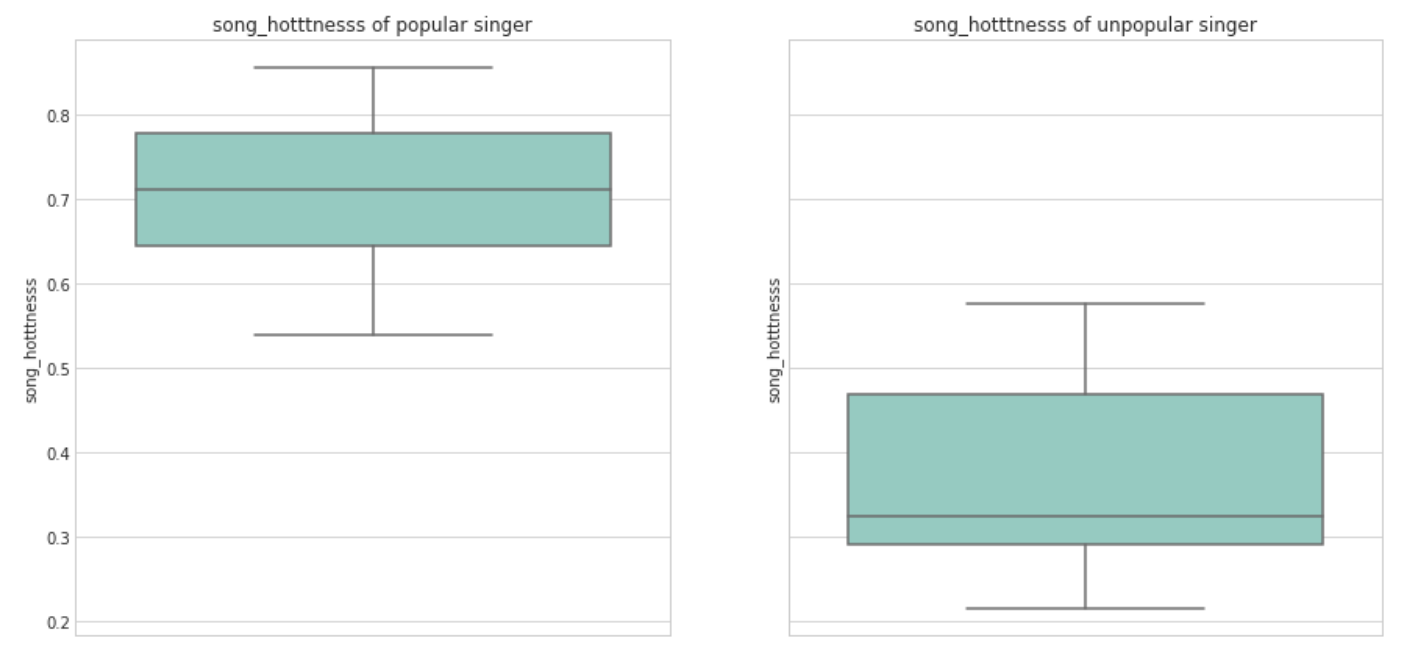
\includegraphics[width=1\linewidth]{img/Q2_2.PNG}
\caption{Song hotness from popular \& unpopular artist}
\end{figure}


\end{exampleblock}

%----------------------------------------------------------------------------------------

\end{column} % End of column 2.2

\end{columns} % End of the split of column 2 - any content after this will now take up 2 columns width

%----------------------------------------------------------------------------------------
%	IMPORTANT RESULT
%----------------------------------------------------------------------------------------

% \begin{alertblock}{Important Result}

% Lorem ipsum dolor \textbf{sit amet}, consectetur adipiscing elit. Sed commodo molestie porta. Sed ultrices scelerisque sapien ac commodo. Donec ut volutpat elit.

% \end{alertblock} 

%----------------------------------------------------------------------------------------

\begin{columns}[t,totalwidth=\twocolwid] % Split up the two columns wide column again

\begin{column}{\onecolwid} % The first column within column 2 (column 2.1)

%----------------------------------------------------------------------------------------
%	MATHEMATICAL SECTION
%----------------------------------------------------------------------------------------

\begin{exampleblock}{The Existence of Herding Bias}
Do you notice that several songs from your playlist are actually from certain artists? We define this phenomenon as \textbf{herding bias} and we measure users' level of herding bias with the following formula:

\vspace{-10mm}  
\begin{equation}
LevelOfHerdingBias = {{\sum_m{p_mI_m}}\over{\sum_m{p_m}}}
\label{eqn:Einstein}
\end{equation}

% \begin{equation}
% \cos^3 \theta =\frac{1}{4}\cos\theta+\frac{3}{4}\cos 3\theta
% \label{eqn:cosfunc}
% \end{equation}
\vspace{-10mm}
$p_m$: total play count of songs from singer m \\ $I_m$: indicator, = 1 if more than 2 songs from artist m and 0 otherwise

% \begin{equation}
% \kappa =\frac{\xi}{E_{\mathrm{max}}} %\mathbb{ZNR}
% \label{eqn:kappa}
% \end{equation}

\begin{figure}
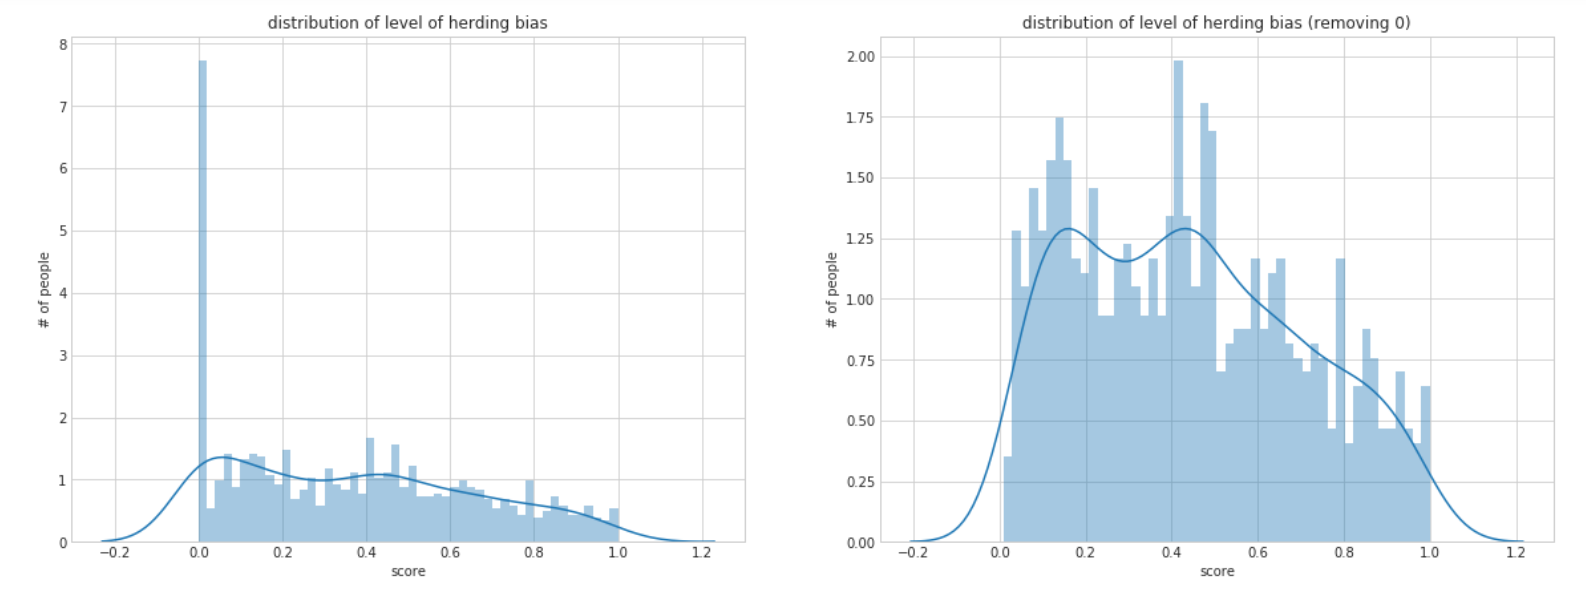
\includegraphics[width=1\linewidth]{img/Q2_1.PNG}
\caption{Distribution of herding bias}
\end{figure}

\vspace{-20mm}
\textbf{160 people out of 1022 people (only 16\%)} do not have herding bias, and the \textbf{median of herding bias is 0.38}.

\end{exampleblock}

%----------------------------------------------------------------------------------------

\end{column} % End of column 2.1
\begin{column}{\sepwid}\end{column} % Empty spacer column

\begin{column}{\onecolwid} % The second column within column 2 (column 2.2)

%----------------------------------------------------------------------------------------
%	RESULTS
%----------------------------------------------------------------------------------------

\begin{exampleblock}{First Performance Is Important}

Do the songs in the first year matter a lot for artist? We choose several popular and unpopular artists during 1995-2000, 2000-2005 and 2005-2010, and observe the song hotness of their songs in their first year.

\begin{figure}
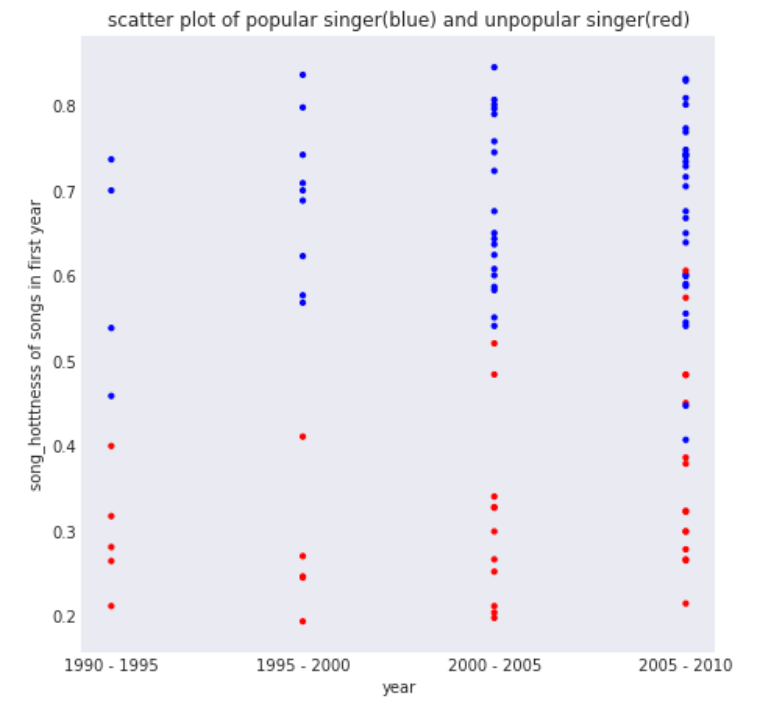
\includegraphics[width=1\linewidth]{img/Q2_3.PNG}
\caption{Song hotness of artist in their 1st year}
\end{figure}

% \begin{table}
% \vspace{2ex}
% \begin{tabular}{l l l}
% \toprule
% \textbf{Treatments} & \textbf{Response 1} & \textbf{Response 2}\\
% \midrule
% Treatment 1 & 0.0003262 & 0.562 \\
% Treatment 2 & 0.0015681 & 0.910 \\
% Treatment 3 & 0.0009271 & 0.296 \\
% \bottomrule
% \end{tabular}
% \caption{Table caption}
% \end{table}

\end{exampleblock}

%----------------------------------------------------------------------------------------

\end{column} % End of column 2.2

\end{columns} % End of the split of column 2

\end{column} % End of the second column

\begin{column}{\sepwid}\end{column} % Empty spacer column

\begin{column}{\onecolwid} % The third column

%----------------------------------------------------------------------------------------
%	CONCLUSION
%----------------------------------------------------------------------------------------

\begin{exampleblock}{Lyrics Distribution}

By exploiting MusiXmatch dataset, we can see many high-ranked words that recall \textbf{feelings} and \textbf{emotions}.

\begin{figure}
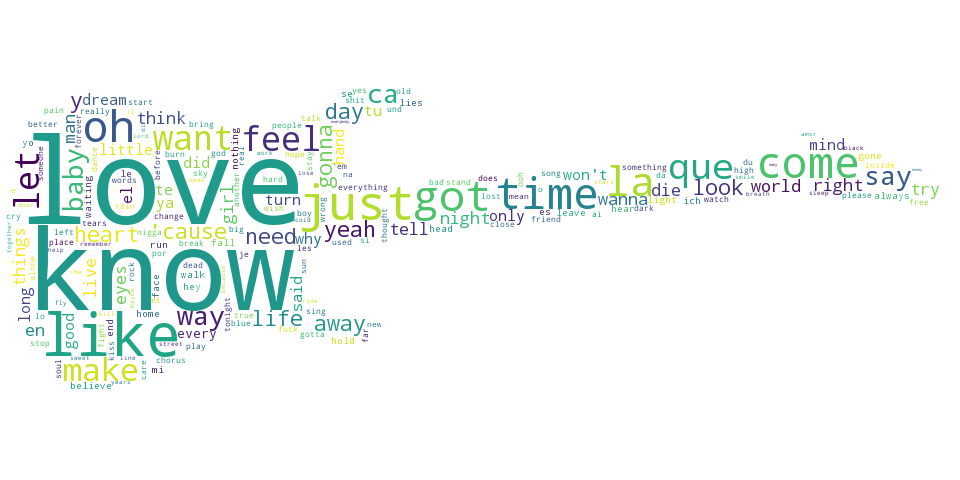
\includegraphics[width=0.9\linewidth]{img/wc3.png}
\caption{Composition of lyrics in both group}
\end{figure}
\end{exampleblock}

\vspace{-20mm}
\begin{exampleblock}{Presence of Slang Words}

"\textit{Slang words}", such as insults, are gathered in frequencies within popular/unpopular songs to give an estimation of the lyrics quality. Are borderline songs more interesting?

\begin{figure}
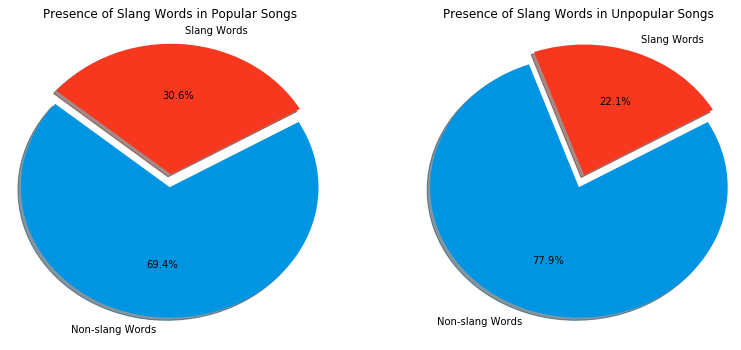
\includegraphics[width=0.8\linewidth]{img/Q3_1.png}
\caption{Ratio of slang words in both group}
\end{figure}
\end{exampleblock}

\vspace{-20mm}
\begin{exampleblock}{Conclusion}
\begin{itemize}
\item People listen to his/her favorite artists. This is proven by important features of random forest classifier and analysis of herding bias phenomenon. "\textit{Rich become Richer}"
\item People care less about slang words in lyrics.
\end{itemize}
\end{exampleblock}

%----------------------------------------------------------------------------------------
%	ADDITIONAL INFORMATION
%----------------------------------------------------------------------------------------

% \begin{exampleblock}{Additional Information}

% Maecenas ultricies feugiat velit non mattis. Fusce tempus arcu id ligula varius dictum. 
% \begin{itemize}
% \item Curabitur pellentesque dignissim
% \item Eu facilisis est tempus quis
% \item Duis porta consequat lorem
% \end{itemize}

% \end{exampleblock}

%----------------------------------------------------------------------------------------
%	REFERENCES
%----------------------------------------------------------------------------------------

% \begin{exampleblock}{References}

% \nocite{*} % Insert publications even if they are not cited in the poster
% \small{\bibliographystyle{unsrt}
% \bibliography{sample}\vspace{1cm}}
% \end{exampleblock}

%----------------------------------------------------------------------------------------
%	ACKNOWLEDGEMENTS
%----------------------------------------------------------------------------------------

%\setbeamercolor{block title}{fg=red,bg=white} % Change the block title color

%\begin{exampleblock}{Acknowledgements}

%\small{\rmfamily{Nam mollis tristique neque eu luctus. Suspendisse rutrum congue nisi sed convallis. Aenean id neque dolor. Pellentesque habitant morbi tristique senectus et netus et malesuada fames ac turpis egestas.}} \\

%\end{exampleblock}

%----------------------------------------------------------------------------------------
%	CONTACT INFORMATION
%----------------------------------------------------------------------------------------

%\setbeamercolor{block alerted title}{fg=black,bg=norange} % Change the alert block title colors
%\setbeamercolor{block alerted body}{fg=black,bg=white} % Change the alert block body colors

\begin{block}{The project}

\begin{itemize}
\item Github: \href{https://github.com/sanadhis/ITT-ADA-2017}{https://github.com/sanadhis/ITT-ADA-2017}
\end{itemize}

\end{block}

% \begin{tabular}{rr}
% \hspace{0.3\linewidth} & 
% 
\includegraphics[width=0.3\linewidth]{img/epfl-logo.jpg}
% \end{tabular}

%----------------------------------------------------------------------------------------

\end{column} % End of the third column

\begin{column}{\sepwid}\end{column} % Empty spacer column

\end{columns} % End of all the columns in the poster

\end{frame} % End of the enclosing frame
%\end{darkframes} % Uncomment for dark theme
\end{document}
